\begin{frame}<1-4>[t]{新知探索}
\begin{campuscanvas}
% Source slide 18, objects 10; visible 2-4
\only<2-4|handout:1>{\node[anchor=north west,inner sep=0,text=black] at (70.000,150.000) {\begin{minipage}[t]{142.500mm}\raggedright\fontsize{16}{24.00}\selectfont \textbf{7. 区间}\end{minipage}};}
% Source slide 18, objects 8; visible 3-4
\only<3-4|handout:1>{\node[anchor=north west,inner sep=0,text=black] at (70.000,235.000) {\begin{minipage}[t]{103.750mm}\raggedright\fontsize{11.5}{17.25}\selectfont 数学里最常用的一类集合叫\red{区间}。\par 设 $a,b\in\mathbf R$，且 $a<b$。\par 所有大于 $a$ 且小于 $b$ 的实数组成\red{开区间}：\[(a,b)=\{x\in\mathbf R\mid a<x<b\}.\]满足 $a\le x\le b$ 的实数组成\red{闭区间} $[a,b]$。\par 类似地，还有左开右闭区间 $(a,b]$ 和左闭右开区间 $[a,b)$。$a,b$ 分别是区间的\red{左端点}和\red{右端点}。\end{minipage}};}
% Source slide 18, objects 9; visible 4
\only<4|handout:1>{\node[anchor=north west,inner sep=0] at (940.000,280.000) {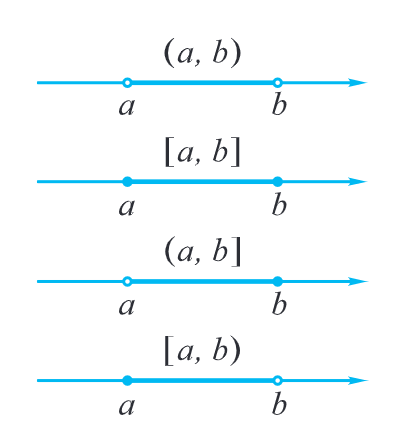
\includegraphics[width=35.000mm,height=40.625mm]{source-media/image26.png}};}
\end{campuscanvas}
\end{frame}
